\documentclass[11pt]{article}

\usepackage{setspace}
\usepackage{inputenc}
\usepackage[margin=1in]{geometry}
\usepackage{subfig}
\usepackage{graphicx}


\title{%
Model Comparison for Bird Species Identification\\
  \large ISyE 6740 - Spring 2022 Project Proposal}
\author{Team Members: Joe Laniado (GTID: 903233267)}


\begin{document}
\begin{singlespace}
\begin{titlepage}
\maketitle
\end{titlepage}
\tableofcontents
\clearpage

\section{Problem Statement}
Ever since computers were created, we have been trying to find ways for them to automate difficult tasks and make our lives easier. Things like finding the shortest path between two places, drawing a three dimensional floor plan for a new skyscraper, or even doing complex mathematical calculations in seconds; have become as trivial as just opening your phone or laptop and asking a question. One of such questions that came up during the late 1960s was: If we give eyes to a computer, would it know what it was looking at? 
Of course the answer was no, but then the goal became to find a way to teach it how to do it. This was the birth of the scientific field of computer vision. This discipline deals with analyzing, processing, and uderstanding visual data in a way which allows a computer to see an image or video, and be able to extract information and make conclusions from it. Using X-ray scans for automatic diagnosis of lung diseases in patients, or collecting quantitive information about the traffic flow of a city using only a camera; are some notable applications of this that are currently in use. \\

After pondering the applications of such computational advancements while doing some bird watching near my home I started to wonder if there could be a way to use computer vision to simplify the process of identifying our feathered friends. I wanted to develop an image classification model that by training it using labeled pictures of different types of birds; if given new input, it could correctly identify which species the new birds belonged to in a quick and efficient way. This process would save me so much time of manual classification of hundreds of pictures of birds in my camera that I just haven't had the time to sit down and check. Fellow local scientists and bird watching enthusiasts have also expressed excitement over the creation of such a model. Furthermore, out in the field spotting a bird could last only a couple of seconds before it flies away, so any time saved on identifiying the species could be used on monitoring other behaviours or collecting scientific information about such a sight. For this a real time video classifier could be used in order to detect and classify the bird before it flies away, although such a project would be a little more advanced than a simple image classifier. \\

Using the different algorithms learned in class, there is a number of ways to approach the development of our bird species identifier. By means of dimensionality reduction, density estimation, traditional classification algorithms, and deep learning; we will build and compare different image classification models until we find the most accurate and efficient approach to correctly identify the species of each bird. We will evaluate each model with a number of performance variables and analyze their behaviour for this specific classification task. Finally, the best model will be selected and further scalability and functionality implementations will be discussed. 

\section{Data Source}

The original dataset consists of pictures from more than 400 different species of birds. This includes 58388 training images, 2000 test images, and 2000 validation images. When it comes to the images themselves; each picture is a 224 x 224 x 3 RGB image in jpg format, and contains only one bird per image. The bird usually takes more than 50\% of the pixels in the image making it convenient for training purposes. All images were collected from the BIRDS 400 dataset found at https://www.kaggle.com/gpiosenka/100-bird-species. One important thing to note is that 85\% of the images are from the male of the species and only 15\% are female, this is due to the male having more colors and features that make them more easily recognizible. Due to the big size of the data 15 different species were selected in order to save time and reduce complexity when implementing each approach for our classifier. More species could be added whenever an optimal classifier is selected. Figure 1 shows the selected species of birds:\\

\begin{figure}[h]
    \centering
    
    \subfloat[Black Broadbill]{
        \label{ref_lael1}
        \includegraphics[width=0.2\textwidth]{data/birds/train/1BLACK YELLOW BROADBILL/001.JPG}
    }
    \subfloat[Flamingo]{
        \label{ref_lbel4}
        \includegraphics[width=0.2\textwidth]{data/birds/train/2FLAMINGO/011.JPG}
    } 
    \subfloat[Bald Eagle]{
        \label{ref_label1}
        \includegraphics[width=0.2\textwidth]{data/birds/train/3BALD EAGLE/019.JPG}
    }
    \subfloat[Annas Hummingbird]{
        \label{ref_label2}
        \includegraphics[width=0.2\textwidth]{data/birds/train/4ANNAS HUMMINGBIRD/006.JPG}
    }
    \subfloat[Scarlet Macaw]{
        \label{ref_label3}
        \includegraphics[width=0.2\textwidth]{data/birds/train/5SCARLET MACAW/016.JPG}
    }\\
    \subfloat[Abbots Babbler]{
        \label{reflabel1}
        \includegraphics[width=0.2\textwidth]{data/birds/train/ABBOTTS BABBLER/013.JPG}
    }
    \subfloat[Abbots Booby]{
        \label{ref_lbel2}
        \includegraphics[width=0.2\textwidth]{data/birds/train/ABBOTTS BOOBY/002.JPG}
    }
    \subfloat[Ground Hornbill]{
        \label{ref_label3}
        \includegraphics[width=0.2\textwidth]{data/birds/train/ABYSSINIAN GROUND HORNBILL/007.JPG}
    }
    \subfloat[Crowned Crane]{
        \label{rf_label3}
        \includegraphics[width=0.2\textwidth]{data/birds/train/AFRICAN CROWNED CRANE/018.JPG}
    } 
    \subfloat[Emerald Cuckoo]{
        \label{ef_label4}
        \includegraphics[width=0.2\textwidth]{data/birds/train/AFRICAN EMERALD CUCKOO/007.JPG}
    }\\
    \subfloat[African Firefinch]{
        \label{ref_lael2}
        \includegraphics[width=0.2\textwidth]{data/birds/train/AFRICAN FIREFINCH/006.JPG}
    }
    \subfloat[Oyster Catcher]{
        \label{ref_label3}
        \includegraphics[width=0.2\textwidth]{data/birds/train/AFRICAN OYSTER CATCHER/009.JPG}
    }
    \subfloat[Alberts Towhee]{
        \label{ref_labl3}
        \includegraphics[width=0.2\textwidth]{data/birds/train/ALBERTS TOWHEE/021.JPG}
    }
    \subfloat[Alexandrine Parakeet]{
        \label{ref_labl4}
        \includegraphics[width=0.2\textwidth]{data/birds/train/ALEXANDRINE PARAKEET/017.JPG}
    }
     \subfloat[Touchan]{
        \label{ref_label4}
        \includegraphics[width=0.2\textwidth]{data/birds/train/6TOUCHAN/013.JPG}
    }
    
    
    \caption{Selected Species}
    \label{selected species}
\end{figure}

The following distribution of pictures applies for each species selected:
\begin{itemize}
\item Training: 120
\item Validation: 5
\item Testing: 5
\end{itemize}

The total distribution ends up being 1800 for training, 75 for validation, and 75 for testing. 

\section{Methodology}
\subsection{Data Pre-Processing}

For efficiency purposes each image was resized to be 64x64x3 pixels, they were then vectorized into the form 1x12,288 and collected into three different matrices. One for training, validation, and testing; where each row represented a singular picture, and each column the pixel values. Each matrix was labeled depending on the species it came from and assembled into dictionaries, where the key-value pair was the species name and the specific matrix respectively. It is important to note that the images were not transformed into grayscale due to color being such an important feature when classifying birds. Furthermore, the disparity between male and female specimens was determined that while it would probably introduce some level of error into our model, in this case it would be used to test the generalization to different cases when performing the classification. At least until more data is available.\\

One area of concern was that due to the high variability between picture design, 120 images per species might not be good enough to capture the complexity of poses and states that the bird could present. This would cause our model to overfit and not generalize well when testing new kinds of pictures. To solve this problem, slight data augmention was implemented to increase the number of samples we had. In order to maintain model efficiency while testing different approches, only rotation and flipping were implemented in order to multiply or training images from 1800 to 7200. Operations like cropping, contrast, translation, and more could be used if more training data is needed for future applications. 

\subsection{Dimensionality Reduction}
The first approach implements a dimensionality reduction technique to find the most representative combination of features for each species and then compare it to a test sample to make a classification. We start by defining our training images as a $M$x$N$ matrix X, where $M$ represents the number of samples and $N$ the number of pixels. To better understand the math behind this technique, it is important to know the following concepts:

\begin{enumerate}
\item The theorem for singular value decomposition states that: $ A_{MxN} = U_{NxN}S_{MxN}V_{NxN}$. Where U and V are orthonormal, $U$ represents the left singular vectors, $S$ the singular values, and $V^T$ the right singular vectors.
\item We also know that for a NxN matrix W, there exists an eigenvector u if:
$$ Wu = \lambda u $$ 
Where $\lambda$ is a scalar that represents the eigenvector of $W$. 
\end{enumerate}

The basic Idea of this approach is that for each species of bird, we will find the $K$ principal components that encompasses it's most representative features by means of singular value decomposition. Using this ``Eigenbirds'' we will then find the projection residual between each test image and all the $K$ principal components for each species. The test image will be labeled as the type of bird that produces the lowest residual in this equation. 

\begin{enumerate}
\item We find the mean image $\mu$ for $X$ and use it to center all of our training images. This will help us calculate the covariance matrix C. We will also divide all the data by 255 to scale for computational efficiency. The following operation can be shown as:
$$ \mu = \frac{1}{m}\sum_{i=0}^{m}X_i $$
$$ X = (X-\mu)/255 $$

\item We can now define our covariance matrix as $ C = XX^T $ which is a symmetrical matrix that can be diagonilized in the form: 
$$ C = ULU^T$$ 
Where U is a matrix of eigenvectors and L is a diagonal matrix with eigenvalues $\lambda_i$- Another approach to calculate the eigenvalues and eigenvectors is to perform SVD on the transpose of our initial matrix X. Furthermore, if we plug our result into C we obtain the relationship between the two methods in calculating our eigenvectors and eigenvalues:
$$ X^T = USV^T  \rightarrow C = USV^TVSU^T = US^2U^T$$
In this case U would represent our principal components and $S^2$ our eigenvalues. 

\item Finally, for each test image $y_i$ and each species $j$; we find the projection residual by:

$$ Z_i = (y_i - \mu_j )/255$$
$$ Projection Residual = || Z_i - U_jU_j^TZ_i ||^2_2 $$

Where $Z_i$ is the centered vector for image $y_i$ using the mean $\mu_j$ of species $j$. After looping through each test image - species combination, the result will be a MxK matrix where each row represents one of $M$ test images and each column the residual when compared to all $K$ species. All is left to do is to find the minimum residual in each row, and that will give us the predicted species for each image. 
\end{enumerate}

The question remains of choosing how many principal components to use when calculating our projection residual. This can be addresed by plotting the variance percentage for each principal component and selecting the ones that explain most of the variance in the data. In this case, after performing SVD for the first 5 species of birds and getting the respective eigenvalues, each one was scaled between 1 and 0 and converted into percentages. They were then plotted in figure 2 to show the explained variance of each principal components for each species. \\

\begin{figure}[h]
    \centering
    
    \subfloat[Black Broadbill]{
        \label{ref_labe1}
        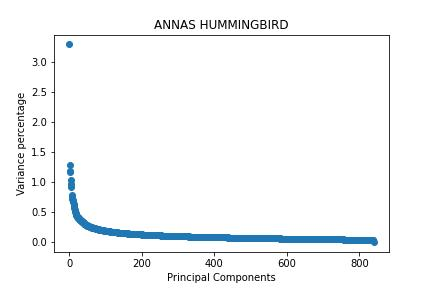
\includegraphics[width=0.33\textwidth]{plots/variance-ANN.jpg}
    }
    \subfloat[Flamingo]{
        \label{ref_labe4}
        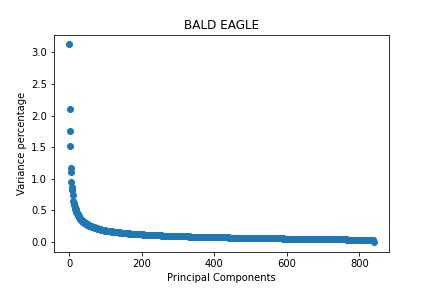
\includegraphics[width=0.33\textwidth]{plots/variance-BAL.jpg}
    } 
    \subfloat[Bald Eagle]{
        \label{ref_labe1}
        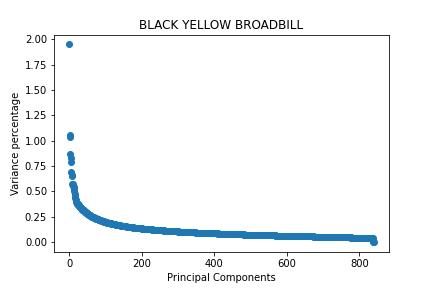
\includegraphics[width=0.33\textwidth]{plots/variance-BLA.jpg}
    }\\
    \subfloat[Annas Hummingbird]{
        \label{ref_labe2}
        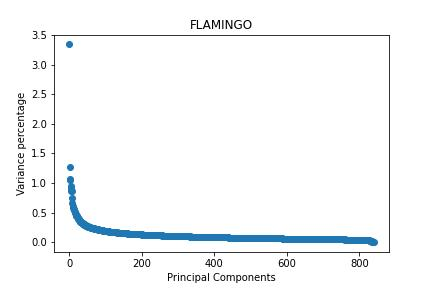
\includegraphics[width=0.33\textwidth]{plots/variance-FLA.jpg}
    }
    \subfloat[Scarlet Macaw]{
        \label{ref_labe3}
        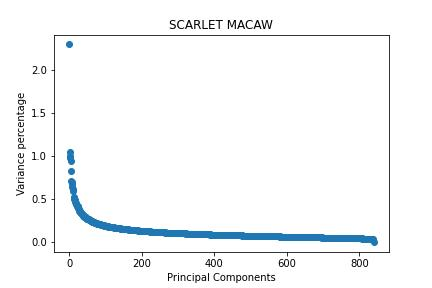
\includegraphics[width=0.33\textwidth]{plots/variance-SCA.jpg}
    }
    
    \caption{Selected Species}
\end{figure}

In all the graphs we can see how most of the variance can be explained by the first N principal components. Using this value we calculated the residuals for each one of our test images. The time in seconds from data input to calculating the labels of each test image, was also calculated in order to see the efficiency of the algorithm. The following were the results:

\begin{itemize}
\item Time for results: 
\item Accuracy: 
\item Precission: 
\item Recall: 
\item F1-score: 
\item Confusion matrix and ROC curve:
\end{itemize}

\subsection{Density Estimation}

A different approach for creating our bird classifier could be using density estimation. If we were to divide all of our training pictures into $n$ different clusters, and group together all the images that look similar enough. We could then use a new input image $x$ and classify it calculating the lowest residual between that image and all the different centroids. Each cluster will be assigned the majority label of that specific cluster as its label. Different measures would need to be taken into account to make sure the model performs well. Things like the homogeneity of each cluster and the overrall accuracy of such a model. More experiments need to be performed to determine if a parametric or non-parametric approach would be best in this case for performing clustering. The advantage of this method is that the number of clusters doesn't need to match the number of species, what would matter most would be the homogeneity of each different cluster with respect to the labels of each training image. This would give us the best opportunity for generalization and high predictive accuracy for future tests. 

\subsection{Classification}

In this step we will be building a number of different models using traditional classification methods. KNN, SVM, Kernel SVM, Logistic Regression, and others will be used to create a classifier for our bird species identifier. We will compare them all and discuss the disadvantages and advantages of using each. Classification and model specific metrics will be presented for technique evaluation, and seeing which one is more efficient for the task. Some of this algorithms might be computationally expensive to use due to the big number of data, if this is the case the results will be presented as such and given as a suboptimal solution to our problem. More experiments will be done regarding this case. 

\subsection{Deep Learning}

Deep learning is a subfield of machine learning that specializes on reproducing the way the human brain thinks to solve certain problems. It does this by using artificial neural networks; a mathematical representation of a composition of neurons signaling to each other. This algorithm has proven to have an endless number of real life applications when it comes to using data to gain insight on an input. In this case, we will implement a variation of this approach called a convolutional neural network. The specific inner workings of this type of network will be discussed and we will do an implementation applied to our training data using the keras library in python. We will use the dropout method to prevent overfitting, and validation to find the optimal parameters for our model. We will use classification metrics to evaluate the quality of our algorithm and the time it takes to produce an output as well. 

\section{Evaluation and Final Results}

In this final section the most meaningful metrics from each one of the 4 applied techniques will be presented and compared. Further discussion on the performance of each and further aplications will be mentioned. Testing with a higher number of data will also be performed at this stage to see how the best technique generalizes when presented with a more real world example. Using our better perfoming approach, we will build our bird species identifier and give the final evaluation metrics of it's implementation. If good results are obtained from initial experiments and no big issues arise while developing each one of the models, a video classifier that takes one frame every $j$ frames and which outputs a label if a bird appears in one of them, might be a good real life implementation of our optimal approach. This will only be done if the scope of this project doesn't prove to be too heavy on one person. If not, scalibility and further possibilities will also be discussed in the conclusion section. 



\end{singlespace}
\end{document}
